\section{Модификация проекта «Выпуклая оболочка»}

\subsection{Постановка задачи}
Требуется модифицировать эталонный проект:
\begin{enumerate}
\item для индуктивного вычисления количества всех острых внутренних углов выпуклой
оболочки~(задача 40).
\item для индуктивного вычисления расстояния от выпуклой оболочки до заданного
стандартного прямоугольника~(Задача 52).
\end{enumerate}
\subsection{Теоретические аспекты}

Задача построения выпуклой оболочки множества точек может быть сформулирована следующим
образом: для множества точек $M$ необходимо найти наименьшее \emph{выпуклое} множество,
включающее $M$. \emph{Выпуклым} будем называть любое множество $M$, удовлетворяющее
условию
$ \forall x_1, x_2 \in M\ [x_1,x_2]\in M.$

\begin{figure}[ht!]
\begin{center}
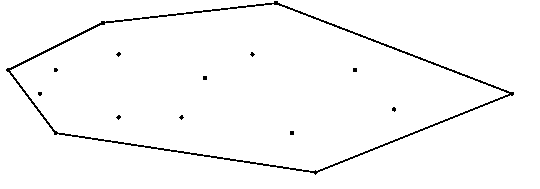
\includegraphics[scale=0.6]{images/conv_a_1}
\end{center}
\vspace*{-8mm}
\caption{Выпуклая оболочка множества точек}\label{fig:convex_hull}
\end{figure}

Пусть $X$~---множество точек на плоскости $\mathbb{R}^2$, $\mathcal{P}$~---
множество всех выпуклых фигур на плоскости. Тогда тройка $(f,g,h)$, где
$f\colon X^* \rightarrow \mathcal{P}$~---
\emph{выпуклая оболочка последовательности точек},
$g\colon X^* \rightarrow \mathbb{N}$~--- \emph{количество острых углов в ней},
$h\colon X^* \rightarrow \mathbb{R}$~---
\emph{расстояние от неё до стандартного прямоугольника}, задаёт индуктивную
функцию $$F\colon X^* \rightarrow \mathcal{P} \times \mathbb{N} \times
\mathbb{R}, F = \begin{pmatrix}f\\ g\\ h\end{pmatrix}.$$
Функция индуктивного перевычисления $G$ представляет собой реализацию следующей
идеи: пусть для некоторой последовательности точек $X^*$ значения $f,g,h$ уже известны.
Тогда при поступлении новой точки $x$ возможны два случая:
либо точка лежит внутри выпуклой оболочки, либо снаружи неё. Если $x$ внутри,
то её можно игнорировать так как она не изменит характеристик выпуклой оболочки.
Рассмотрим случай когда она находится снаружи: хорошей
моделью для дополнения выпуклой оболочки будет \emph{освещённость} рёбер из
добавляемой точки.
 \ref{fig:conv_light}.
\begin{figure}[ht!]
\begin{center}
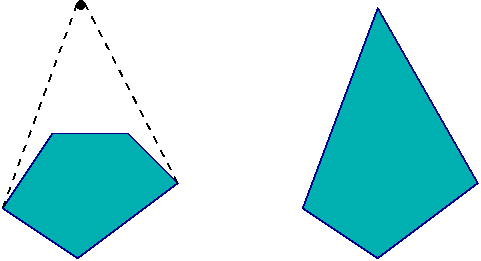
\includegraphics[scale=0.6]{images/conv_a_2}
\end{center}
\vspace*{-8mm}
\caption{Изменение выпуклой оболочки при добавлении точки}\label{fig:conv_light}
\end{figure}

Для получения новой оболочки необходимо удалить все освещённые рёбра, а концы
оставшейся ломаной соединить двумя новыми рёбрами с добавляемой точкой $x$.
Если добавляемая точка лежит на продолжении одного из рёбер, то оболочка должна
измениться, поэтому ребро, на продолжении которого лежит точка $x$ мы также будем
считать освещённым.
\newpage
